\documentclass[11pt,a4paper]{article}
\usepackage[margin=2.2cm]{geometry}
\usepackage[T1]{fontenc}
\usepackage{lmodern}
\usepackage{microtype}
\usepackage{xcolor}
\usepackage{booktabs}
\usepackage{float}
\usepackage{enumitem}
\usepackage{tikz}
\usetikzlibrary{shapes.geometric,arrows.meta,positioning,calc,fit}
\usepackage[hidelinks]{hyperref}

\setlist{itemsep=2pt,topsep=4pt}
\setlength{\parskip}{5pt}
\setlength{\parindent}{0pt}

% ---------- flowchart styles ----------
\definecolor{startc}{HTML}{D8EEDB}
\definecolor{stepc}{HTML}{DDE8F6}
\definecolor{askc}{HTML}{FCEBC6}
\definecolor{stopc}{HTML}{F6D5D5}
\tikzset{
  flow/.style={node distance=6mm and 9mm, every node/.style={font=\small}},
  start/.style={rectangle, rounded corners=9pt, draw, fill=startc, minimum height=8mm,
                text width=#1, align=center, inner sep=4pt},
  start/.default=38mm,
  step/.style={rectangle, draw, fill=stepc, minimum height=8mm, text width=#1,
               align=center, inner sep=4pt},
  step/.default=52mm,
  ask/.style={diamond, aspect=2.4, draw, fill=askc, text width=#1, align=center, inner sep=1pt},
  ask/.default=30mm,
  stop/.style={rectangle, rounded corners=9pt, draw, fill=stopc, minimum height=8mm,
               text width=#1, align=center, inner sep=4pt},
  stop/.default=38mm,
  arr/.style={-{Stealth[length=2.4mm]}, thick},
  lab/.style={font=\footnotesize\itshape, inner sep=1pt},
}

\title{\textbf{Two Robot Arms That Build With LEGO}\\[4pt]
\large How the project works, explained in simple words}
\author{ISDN Robotic LEGO Assembly project}
\date{November 2026}

\begin{document}
\maketitle

\begin{center}
\fbox{\parbox{0.9\linewidth}{\small
\textbf{What this report is.} A plain-language tour of the project: how a
drawing becomes a list of bricks, how the robots decide the order and when one
needs to hold the model steady, how the computer pretends to be the real world,
and how each arm picks up, carries and clicks in every brick without bumping into
anything. Each part has a flowchart: start at the green box, follow the arrows,
answer the yellow questions with ``yes'' or ``no'', and stop at the red box.}}
\end{center}

\tableofcontents
\newpage

% =====================================================================
\section{The big picture}

Imagine you want two robot arms to build a LEGO model for you. You draw the
model from the front and from the side. The computer then has to answer four
questions:

\begin{enumerate}
\item \textbf{What bricks make this shape?} (the \emph{blueprint})
\item \textbf{In what order should they go on?} (the \emph{plan})
\item \textbf{Will the model wobble or break while a brick is pushed on?} If so,
      the other arm holds it steady (a \emph{support}).
\item \textbf{How does each arm actually do it?} Pick up, carry, place, check,
      and never crash into the other arm (the \emph{control}).
\end{enumerate}

Everything happens inside a computer \emph{simulation}: a pretend world where
bricks fall, slide and click like real ones. Two robot arms (called A and B)
each build their own model at the same time, side by side, and help each other
when one model needs holding.

\begin{figure}[H]
\centering
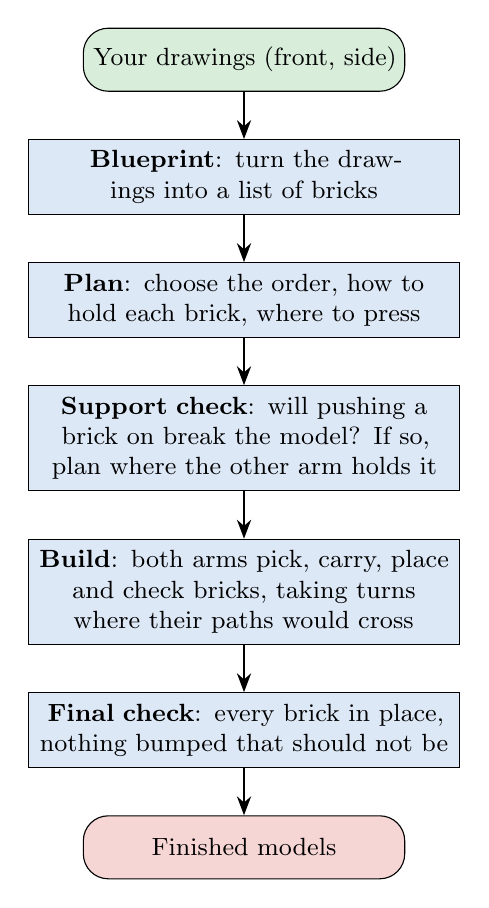
\begin{tikzpicture}[flow]
\node[start] (a) {Your drawings (front, side)};
\node[step, below=of a] (b) {\textbf{Blueprint}: turn the drawings into a list of bricks};
\node[step, below=of b] (c) {\textbf{Plan}: choose the order, how to hold each brick, where to press};
\node[step, below=of c] (d) {\textbf{Support check}: will pushing a brick on break the model? If so, plan where the other arm holds it};
\node[step, below=of d] (e) {\textbf{Build}: both arms pick, carry, place and check bricks, taking turns where their paths would cross};
\node[step, below=of e] (f) {\textbf{Final check}: every brick in place, nothing bumped that should not be};
\node[stop, below=of f] (g) {Finished models};
\foreach \u/\v in {a/b,b/c,c/d,d/e,e/f,f/g} \draw[arr] (\u) -- (\v);
\end{tikzpicture}
\caption{The whole project, from drawing to finished model.}
\end{figure}

% =====================================================================
\section{Making the blueprint: from drawing to bricks}

\subsection{The idea in simple words}

LEGO bricks sit on an invisible 3D grid. One step sideways is one stud
(8\,mm) and one step up is one brick height (9.6\,mm). So we first build the
model out of tiny grid cubes, and then cover those cubes with real bricks.

\textbf{Step 1 -- Read the drawings.} Each drawing is a dark shape on a light
background (or the opposite). The computer finds the shape and cuts away the
empty border.

\textbf{Step 2 -- Fit the drawing onto the grid.} You say how many studs wide
the model is. From that, the computer works out how many layers tall it must
be, using the real stud and brick sizes. Each grid square is marked ``full'' if
more than half of it is dark in the drawing.

\textbf{Step 3 -- Carve the model, like a shadow puzzle.} Start with a solid
block of grid cubes. Look at it from the front: any cube outside the front
shape is removed. Look from the side: any cube outside the side shape is
removed. What is left matches every drawing. (A hidden hole that no drawing can
see is simply filled in.)

\textbf{Step 4 -- Cover the cubes with bricks, one layer at a time, from the
bottom.} The computer can use these bricks: 2$\times$6, 2$\times$4,
2$\times$3, 2$\times$2, 1$\times$6, 1$\times$4, 1$\times$2 and 1$\times$1. In
each layer:
\begin{itemize}
\item Cells that hang over empty space are covered first, by a brick that sits on
      as many bricks below as possible. That is what ties the two legs of an arch
      together.
\item Every brick must sit on at least one brick below. If a cell cannot be
      reached that way, the shape overhangs too far and the computer says so.
\item When there is a choice, it prefers a brick that does not put a joint right
      on top of a joint below (like a brick wall), then bigger bricks, then
      bricks that point the other way from the layer below (crossing layers makes
      the model stronger).
\end{itemize}

\textbf{Step 5 -- Number the bricks} in the order they will be built.

\begin{figure}[H]
\centering
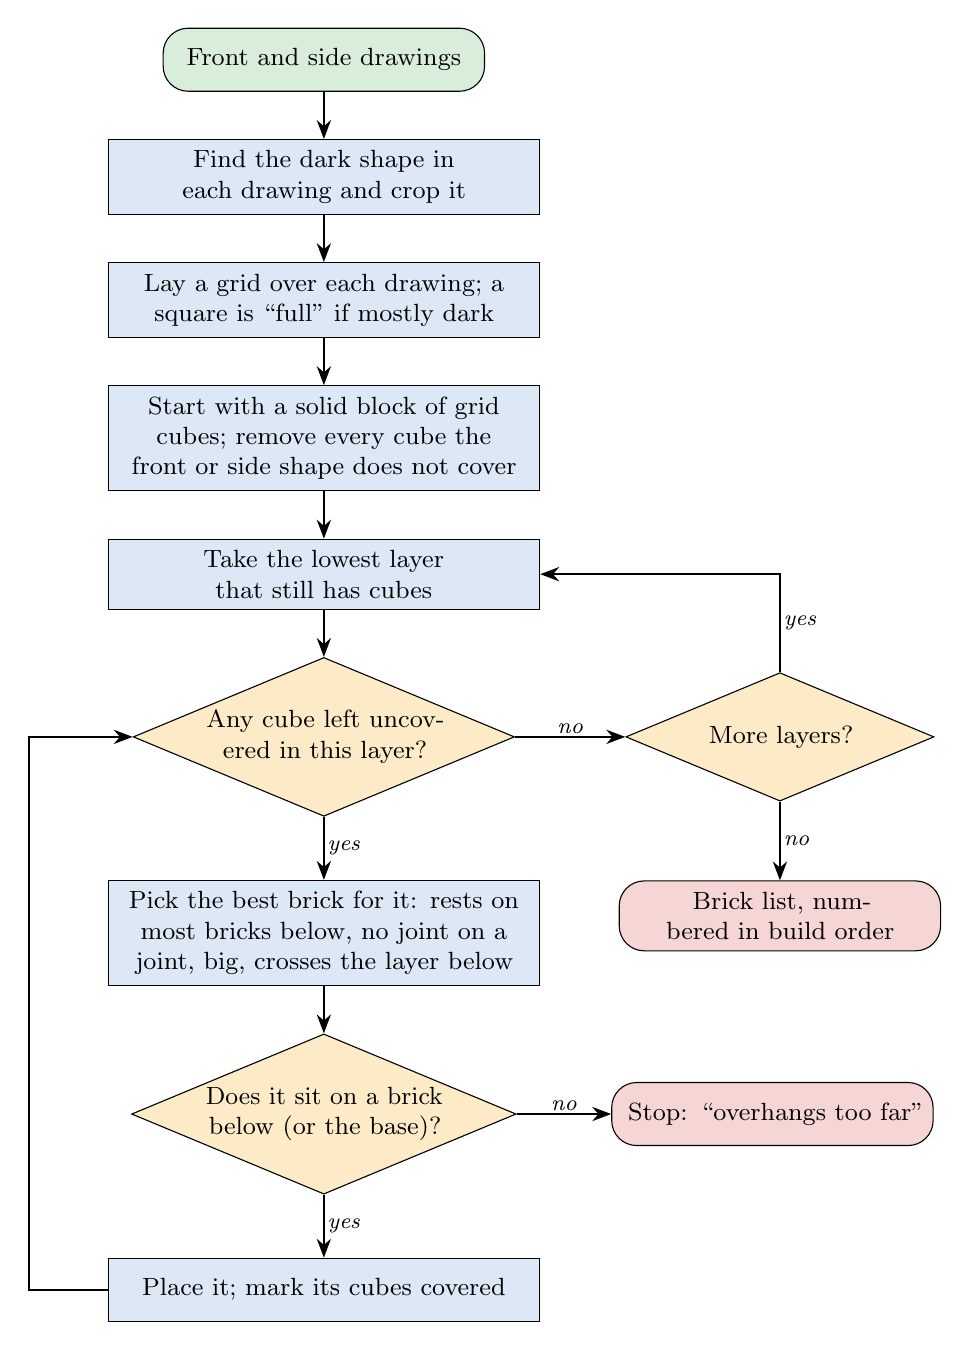
\begin{tikzpicture}[flow]
\node[start] (s) {Front and side drawings};
\node[step, below=of s] (m) {Find the dark shape in each drawing and crop it};
\node[step, below=of m] (g) {Lay a grid over each drawing; a square is ``full'' if mostly dark};
\node[step, below=of g] (c) {Start with a solid block of grid cubes; remove every cube the front or side shape does not cover};
\node[step, below=of c] (l) {Take the lowest layer that still has cubes};
\node[ask, below=of l] (q1) {Any cube left uncovered in this layer?};
\node[step, below=of q1, yshift=-2mm] (pick) {Pick the best brick for it: rests on most bricks below, no joint on a joint, big, crosses the layer below};
\node[ask, below=of pick] (q2) {Does it sit on a brick below (or the base)?};
\node[stop, right=12mm of q2] (bad) {Stop: ``overhangs too far''};
\node[step, below=of q2, yshift=-2mm] (put) {Place it; mark its cubes covered};
\node[ask, right=14mm of q1] (q3) {More layers?};
\node[stop, below=of q3, yshift=-4mm] (done) {Brick list, numbered in build order};
\draw[arr] (s)--(m); \draw[arr] (m)--(g); \draw[arr] (g)--(c); \draw[arr] (c)--(l); \draw[arr] (l)--(q1);
\draw[arr] (q1)-- node[lab, right]{yes} (pick);
\draw[arr] (pick)--(q2);
\draw[arr] (q2)-- node[lab, above]{no} (bad);
\draw[arr] (q2)-- node[lab, right]{yes} (put);
\draw[arr] (put.west) -- ++(-10mm,0) |- (q1.west);
\draw[arr] (q1)-- node[lab, above]{no} (q3);
\draw[arr] (q3.north) |- node[lab, pos=.25, right]{yes} (l.east);
\draw[arr] (q3)-- node[lab, right]{no} (done);
\end{tikzpicture}
\caption{Turning drawings into a list of bricks.}
\end{figure}

% =====================================================================
\section{Making the plan: order, grip and press}

The blueprint says \emph{which} bricks. The plan says \emph{how} to build them.
For every brick the plan writes down one ``step'':

\begin{itemize}
\item \textbf{When.} Bricks go on from the bottom layer up. A brick may only be
      placed once the bricks under it are there. Inside a layer, square
      2$\times$2 bricks go first, so the fingers that hold them do not rub
      against a neighbour.
\item \textbf{Where.} The exact spot and turn of the brick on the base plate,
      and a spot just above it (``hover point'') where the arm stops before going
      down.
\item \textbf{How to hold it.} The gripper has two flat fingers that squeeze two
      opposite sides of the brick. The plan picks the pair of sides where the
      fingers touch the fewest bricks already standing next to it, and how wide
      to open.
\item \textbf{Where to press.} If only part of a brick sits on bricks below (an
      overhang, like a shelf), pressing it in the middle could tip it. So the plan
      slides the grip toward the part that is supported, choosing the spot that
      puts the least strain on the model.
\end{itemize}

\textbf{Tight spots.} Sometimes a brick's neighbours are so close that the
fingers cannot reach down beside it. Two things help:
\begin{itemize}
\item \textbf{Reorder small bricks.} If a tiny 1$\times$1 brick would end up boxed
      in, its layer is rebuilt smallest-bricks-first, so the 1$\times$1 goes in
      while there is still room for the fingers. (A dropped 1$\times$1 rolls off
      its single stud and falls over, so it must be held all the way down.)
\item \textbf{Grip fallbacks.} The arm tries grips in a fixed order: the planned
      one, the other pair of sides, then holding the brick a little off-centre,
      nearest first. If none fits, it uses \emph{drop-and-press}: let go of the
      brick just above its spot, then push it down with the closed fingertips.
\end{itemize}

\begin{figure}[H]
\centering
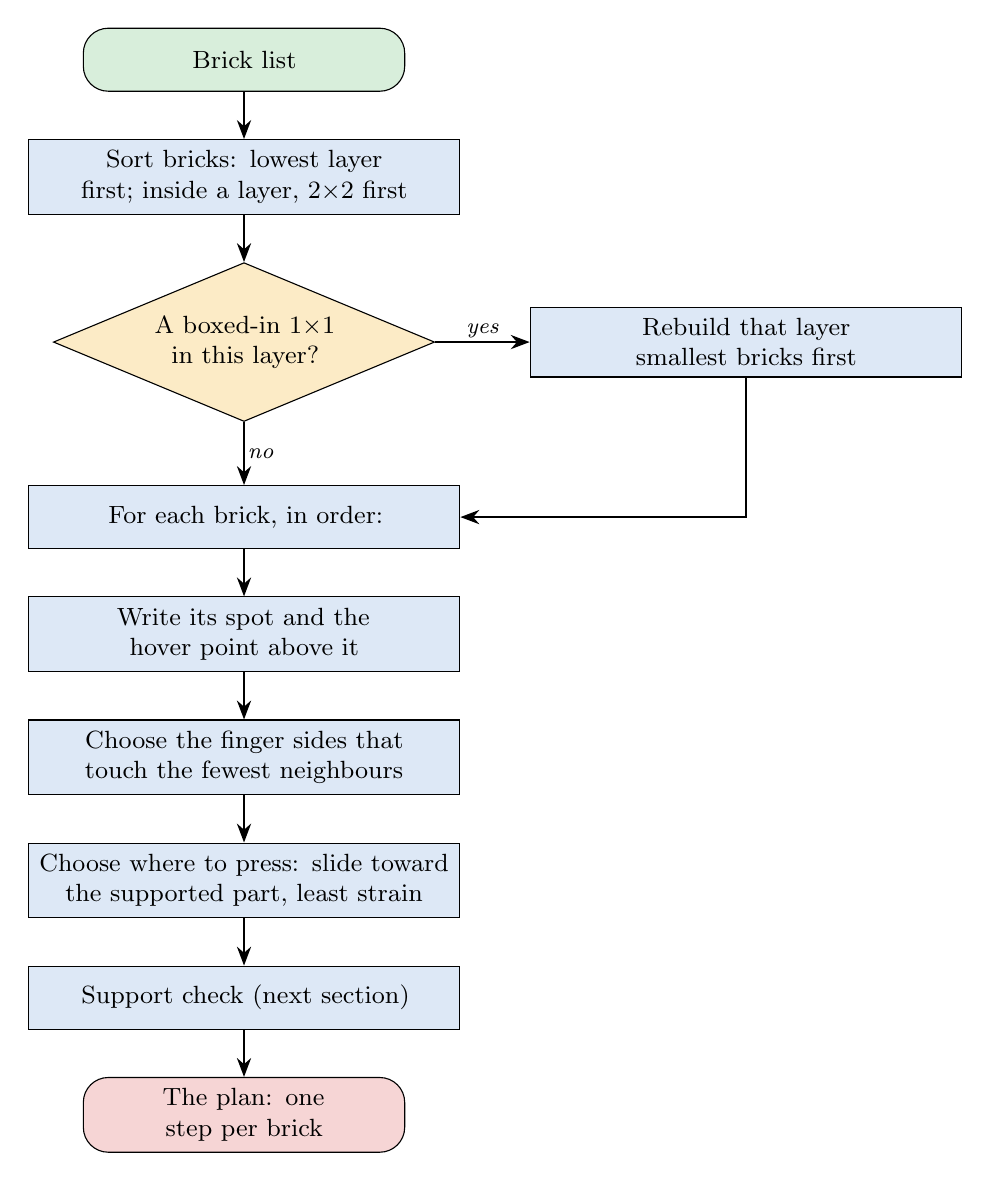
\begin{tikzpicture}[flow]
\node[start] (s) {Brick list};
\node[step, below=of s] (o) {Sort bricks: lowest layer first; inside a layer, 2$\times$2 first};
\node[ask, below=of o] (q1) {A boxed-in 1$\times$1 in this layer?};
\node[step, right=12mm of q1] (r) {Rebuild that layer smallest bricks first};
\node[step, below=of q1, yshift=-2mm] (e) {For each brick, in order:};
\node[step, below=of e] (w) {Write its spot and the hover point above it};
\node[step, below=of w] (h) {Choose the finger sides that touch the fewest neighbours};
\node[step, below=of h] (p) {Choose where to press: slide toward the supported part, least strain};
\node[step, below=of p] (b) {Support check (next section)};
\node[stop, below=of b] (d) {The plan: one step per brick};
\draw[arr] (s)--(o); \draw[arr] (o)--(q1);
\draw[arr] (q1)-- node[lab, above]{yes} (r);
\draw[arr] (r) |- (e.east);
\draw[arr] (q1)-- node[lab, right]{no} (e);
\foreach \u/\v in {e/w,w/h,h/p,p/b,b/d} \draw[arr] (\u)--(\v);
\end{tikzpicture}
\caption{Turning a brick list into a step-by-step plan.}
\end{figure}

% =====================================================================
\section{Does the model need a helping hand?}

\subsection{Why a model can break while you build it}

LEGO bricks hold together because the studs squeeze into the brick above. Each
stud holds about 11.3 newtons before it pops off (a newton is roughly the weight
of a small apple). Pushing a new brick on needs about 8.9 newtons per stud. So
when the arm presses a brick onto a tall or overhanging part, that push can lever
another joint apart, like pressing on the end of a diving board.

\subsection{How the computer checks}

For every step, the computer imagines the press. It uses 1.3 times the normal
push, to be on the safe side. Then it works out how hard every joint in the
model is being pulled or bent. Each joint gets a score: its load divided by its
strength. A score of 1 means ``right at breaking point''.

\begin{itemize}
\item It multiplies the score by a safety factor of 1.5. If the result is 1 or
      more, that step \textbf{needs support}.
\item Then it finds the \textbf{weakest joint}, the one closest to breaking.
\item It tries ways for the other arm to grip the model near that joint. The
      helper's fingers squeeze the bricks on both sides of the weak joint, so the
      push goes into the robot instead of through the joint. It keeps the grip
      that gives the lowest score.
\item It checks that the two hands fit: the helper leans its hand away (45, 60
      or 75 degrees) so it does not get in the way of the placing hand.
\item If no grip makes the step safe, planning stops with a clear message.
\end{itemize}

\begin{figure}[H]
\centering
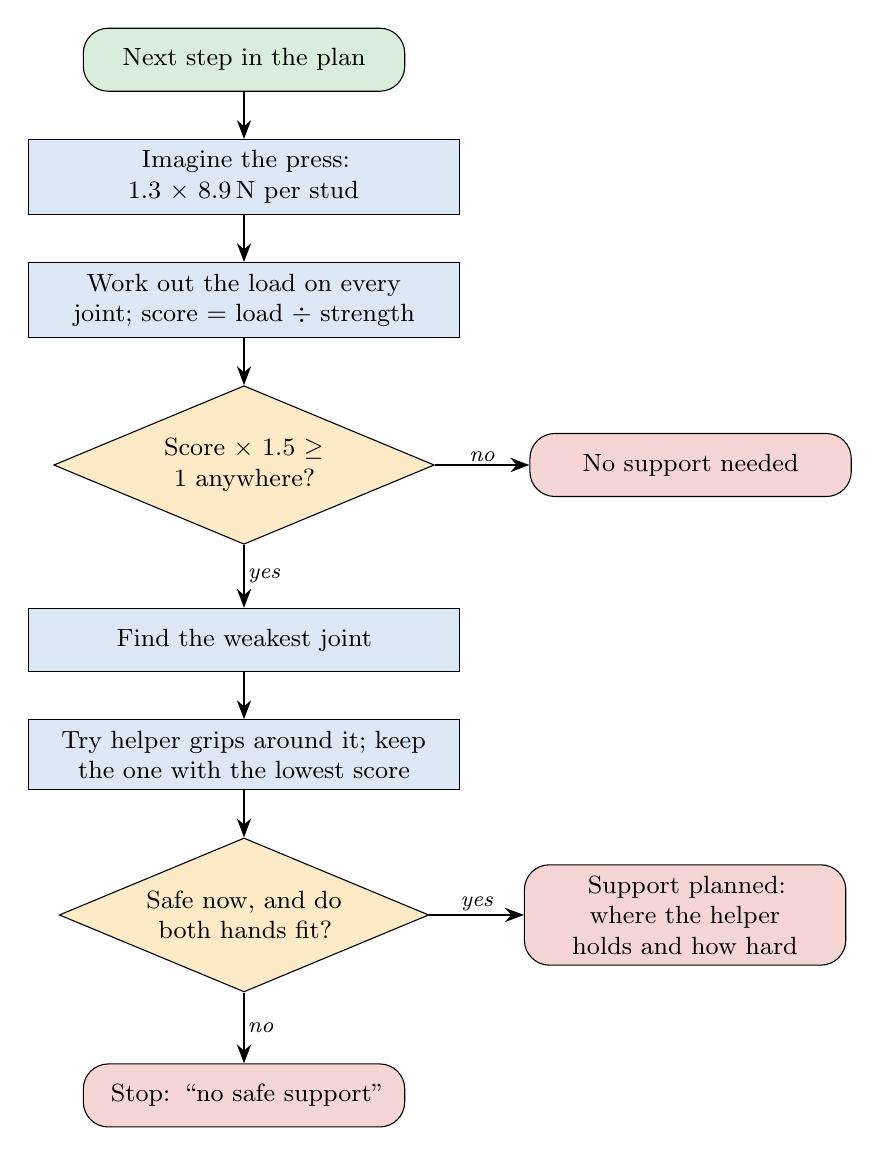
\begin{tikzpicture}[flow]
\node[start] (s) {Next step in the plan};
\node[step, below=of s] (f) {Imagine the press: 1.3 $\times$ 8.9\,N per stud};
\node[step, below=of f] (j) {Work out the load on every joint; score = load $\div$ strength};
\node[ask, below=of j] (q1) {Score $\times$ 1.5 $\geq$ 1 anywhere?};
\node[stop, right=12mm of q1] (no) {No support needed};
\node[step, below=of q1, yshift=-2mm] (w) {Find the weakest joint};
\node[step, below=of w] (g) {Try helper grips around it; keep the one with the lowest score};
\node[ask, below=of g] (q2) {Safe now, and do both hands fit?};
\node[stop, right=12mm of q2] (yes) {Support planned: where the helper holds and how hard};
\node[stop, below=of q2, yshift=-3mm] (fail) {Stop: ``no safe support''};
\draw[arr] (s)--(f); \draw[arr] (f)--(j); \draw[arr] (j)--(q1);
\draw[arr] (q1)-- node[lab, above]{no} (no);
\draw[arr] (q1)-- node[lab, right]{yes} (w);
\draw[arr] (w)--(g); \draw[arr] (g)--(q2);
\draw[arr] (q2)-- node[lab, above]{yes} (yes);
\draw[arr] (q2)-- node[lab, right]{no} (fail);
\end{tikzpicture}
\caption{Deciding whether a step needs the other arm to hold the model.}
\end{figure}

% =====================================================================
\section{The pretend world: how bricks are simulated}

The project does not use real robots yet. It runs a \textbf{physics
simulation}: a program that moves everything the way gravity, pushes and
bumps would move it in real life. It runs on the computer's graphics card,
which is very fast at doing many small sums at once.

\begin{itemize}
\item \textbf{Time in small steps.} The world moves forward 60 times a second,
      and each of those is split into 16 even smaller steps, so fast bumps are
      not missed.
\item \textbf{Two shapes per brick.} Each brick has a detailed shape with
      studs (what you see and what the fingers touch), plus a few hidden simple
      blocks: a top slab, four walls and one cylinder per stud. The computer uses
      the hidden blocks to work out when bricks touch, because simple shapes are
      quick and reliable.
\item \textbf{The click.} When a brick is in the right spot (see
      Section~\ref{sec:done}), invisible ``glue'' joints switch on between it and
      the bricks under it. From then on it holds like a clicked-in brick.
\item \textbf{Breaking.} Every glue joint keeps checking how hard it is being
      pulled or bent. If that is more than the studs can hold, two checks in a row,
      the joint breaks and the build stops, just as a real brick would pop off.
\item \textbf{The robots.} Two Franka robot arms with two-finger grippers. Each
      joint of the arm is driven like a stiff spring toward the angle it is told.
\end{itemize}

\textbf{Two versions of the studs.} In the normal version the hidden stud
cylinders leave a small gap (0.6\,mm each side), so a brick slides onto the
studs by its own weight and the ``click'' is the check plus the glue. The
\textbf{stud-fit version} (switched on with \texttt{--stud-fit}) is more like
real LEGO. A brick stops on top of the studs and only goes down when it is
pushed with 8.9\,N per stud. The arm has to press it in, using a stronger,
stiffer press from above.

\begin{figure}[H]
\centering
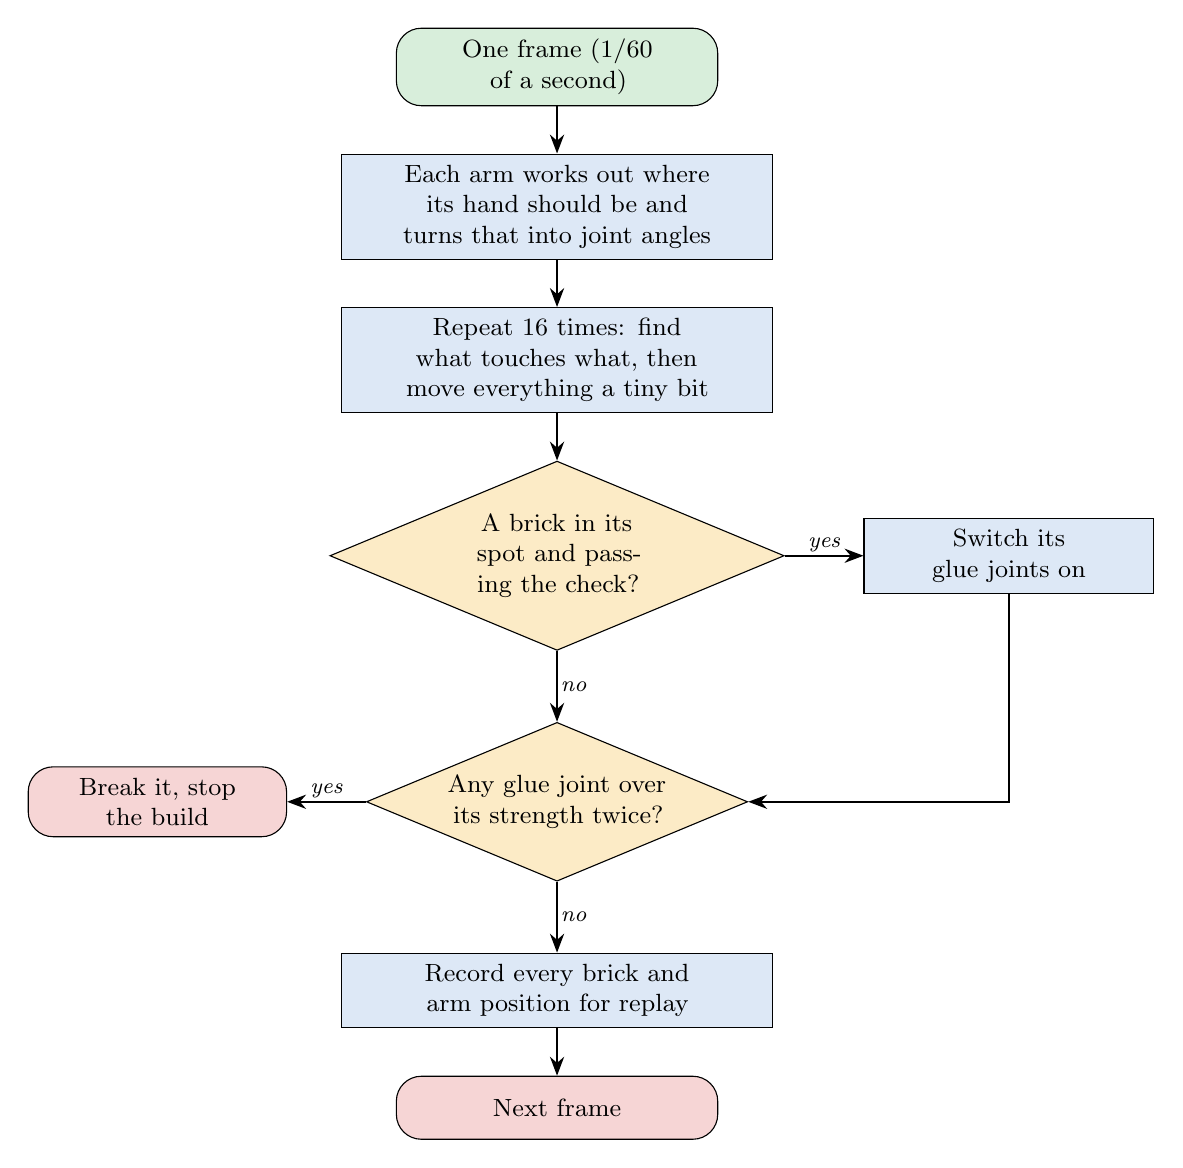
\begin{tikzpicture}[flow]
\node[start] (s) {One frame (1/60 of a second)};
\node[step, below=of s] (c) {Each arm works out where its hand should be and turns that into joint angles};
\node[step, below=of c] (t) {Repeat 16 times: find what touches what, then move everything a tiny bit};
\node[ask, below=of t] (q1) {A brick in its spot and passing the check?};
\node[step=34mm, right=10mm of q1] (glue) {Switch its glue joints on};
\node[ask, below=of q1, yshift=-3mm] (q2) {Any glue joint over its strength twice?};
\node[stop=30mm, left=10mm of q2] (brk) {Break it, stop the build};
\node[step, below=of q2, yshift=-3mm] (r) {Record every brick and arm position for replay};
\node[stop, below=of r] (n) {Next frame};
\draw[arr] (s)--(c); \draw[arr] (c)--(t); \draw[arr] (t)--(q1);
\draw[arr] (q1)-- node[lab, above]{yes} (glue);
\draw[arr] (glue) |- (q2.east);
\draw[arr] (q1)-- node[lab, right]{no} (q2);
\draw[arr] (q2)-- node[lab, above]{yes} (brk);
\draw[arr] (q2)-- node[lab, right]{no} (r);
\draw[arr] (r)--(n);
\end{tikzpicture}
\caption{What the pretend world does every frame.}
\end{figure}

% =====================================================================
\section{Control: how the arms do the work}

\subsection{Picking up and placing a brick}

Each brick waits in its own spot on the table, the ``feeder''. To place it,
the arm follows a fixed list of moves:

\begin{enumerate}
\item \textbf{Go to the feeder} and stop high above the brick.
\item \textbf{Go down}, close the fingers on the chosen sides, and \textbf{lift}.
\item \textbf{Carry} the brick high above everything, to the hover point over its spot.
\item \textbf{Go down slowly} toward the spot. On the way the arm watches where the
      \emph{brick} really is, not just its own hand, and nudges itself by up to
      4\,mm so the brick lands exactly over the studs. (A brick can slip a little
      in the fingers, so the brick is what matters.)
\item If the spot is a tight slot, \textbf{wiggle} it gently (small side-to-side
      and rocking moves) so it slides in.
\item \textbf{Check the brick} (Section~\ref{sec:done}). If it passes, it clicks in.
\item \textbf{Open the fingers} while rising a little, \textbf{lift away}, and go
      to a safe resting pose (``park'').
\end{enumerate}

\begin{figure}[H]
\centering
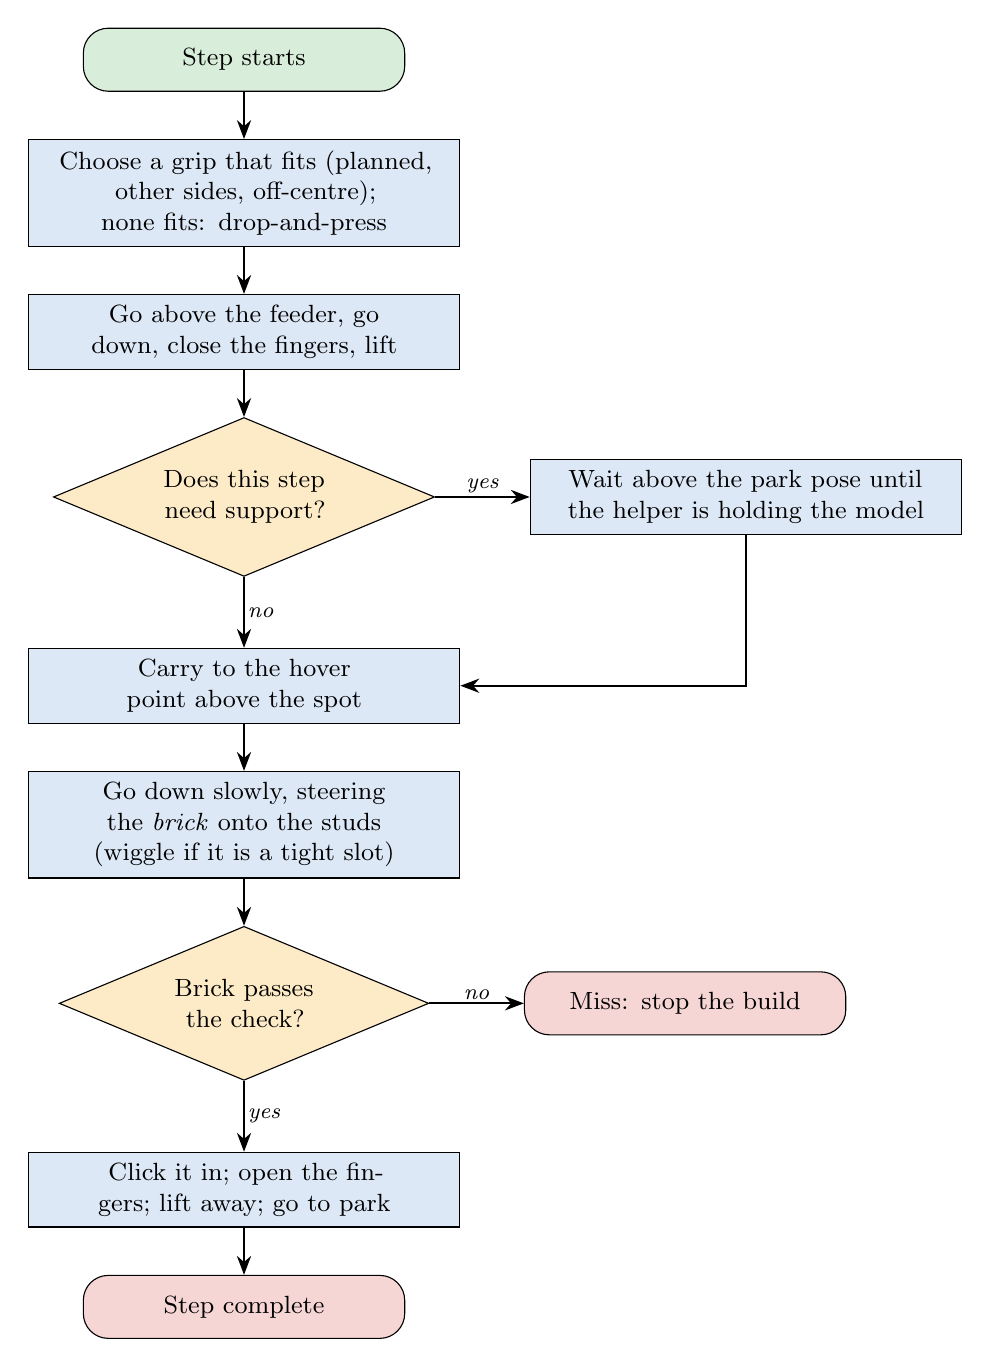
\begin{tikzpicture}[flow]
\node[start] (s) {Step starts};
\node[step, below=of s] (g) {Choose a grip that fits (planned, other sides, off-centre); none fits: drop-and-press};
\node[step, below=of g] (f) {Go above the feeder, go down, close the fingers, lift};
\node[ask, below=of f] (q1) {Does this step need support?};
\node[step, right=12mm of q1] (w) {Wait above the park pose until the helper is holding the model};
\node[step, below=of q1, yshift=-3mm] (c) {Carry to the hover point above the spot};
\node[step, below=of c] (d) {Go down slowly, steering the \emph{brick} onto the studs (wiggle if it is a tight slot)};
\node[ask, below=of d] (q2) {Brick passes the check?};
\node[stop, right=12mm of q2] (m) {Miss: stop the build};
\node[step, below=of q2, yshift=-3mm] (o) {Click it in; open the fingers; lift away; go to park};
\node[stop, below=of o] (e) {Step complete};
\draw[arr] (s)--(g); \draw[arr] (g)--(f); \draw[arr] (f)--(q1);
\draw[arr] (q1)-- node[lab, above]{yes} (w);
\draw[arr] (w) |- (c.east);
\draw[arr] (q1)-- node[lab, right]{no} (c);
\draw[arr] (c)--(d); \draw[arr] (d)--(q2);
\draw[arr] (q2)-- node[lab, above]{no} (m);
\draw[arr] (q2)-- node[lab, right]{yes} (o);
\draw[arr] (o)--(e);
\end{tikzpicture}
\caption{Pick and place, one brick.}
\end{figure}

\subsection{Drop-and-press and the stud-fit press}

When the fingers cannot reach down beside a brick, the arm lowers it only until
the fingers are still clear of the neighbours, waits a moment, and lets go. The
brick drops onto the studs. Then the arm closes its fingers into a ``fist'',
comes down on top of the brick, and pushes it into place.

In the stud-fit version every brick is pressed this way, because the fingers
can only squeeze gently (the brick would slip at about 3\,N). The press is
careful:
\begin{itemize}
\item the push grows smoothly to 1.3 times what the studs need;
\item the arm (and a helping arm, if any) goes stiff while pressing, so the hand
      does not slide off;
\item it presses where the plan says, not where an old guess was;
\item the push stops the moment the brick goes in. The computer then waits a
      quarter of a second for the model to settle before checking it.
\end{itemize}

\subsection{Finding a path: route planning}

Moving a robot arm is like steering a long, bendy snake. To get from one place
to another without hitting anything, the arm uses a \textbf{route planner}
(called cuRobo). You can think of it as a satnav for the arm's seven joints.

\begin{itemize}
\item The planner is told about everything in the way: the two models, the base
      plates, the table, the bricks waiting in the feeders, and the other arm.
      Each of these is a simple box shape.
\item It searches for a smooth set of joint movements that keeps every part of
      the arm, and the brick it carries, away from all of those boxes.
\item For the short, careful moves at the end (going down onto the studs, letting
      go, lifting off) the arm moves its hand in a straight line instead.
\item If no route is found while the other arm is busy, it waits and tries again.
\end{itemize}

\subsection{Not bumping into things: safety bubbles}

The computer pictures each arm as a chain of \textbf{bubbles} (spheres) that
cover it like bubble wrap, and every obstacle as a box.

\begin{itemize}
\item \textbf{Every command is checked.} Before an arm is told to move, the
      computer checks the bubbles at the new position. Every bubble must stay at
      least 1\,mm from every box, except the ones it is meant to touch: the brick
      in its own hand, and the bricks right next to the spot while pressing.
      Anything closer stops that arm.
\item \textbf{The two arms share the space by booking it.} Before an arm starts
      a move, it ``books'' the space its bubbles will sweep through. If that
      space overlaps space the other arm has booked, it waits until the other
      arm is done. If both ask at the very same moment, arm A goes first and B
      waits its turn.
\item \textbf{Staying inside the booking.} For the short straight-line moves, the
      arm books a little extra room around its hand. If the hand ever leaves its
      booked space, the arm stops.
\item \textbf{Touch checks.} Every contact in the pretend world is sorted into
      ``meant to happen'' (fingers on the held brick, a brick on its studs) or
      ``not meant to happen''. The second kind fails the final check.
\end{itemize}

\begin{figure}[H]
\centering
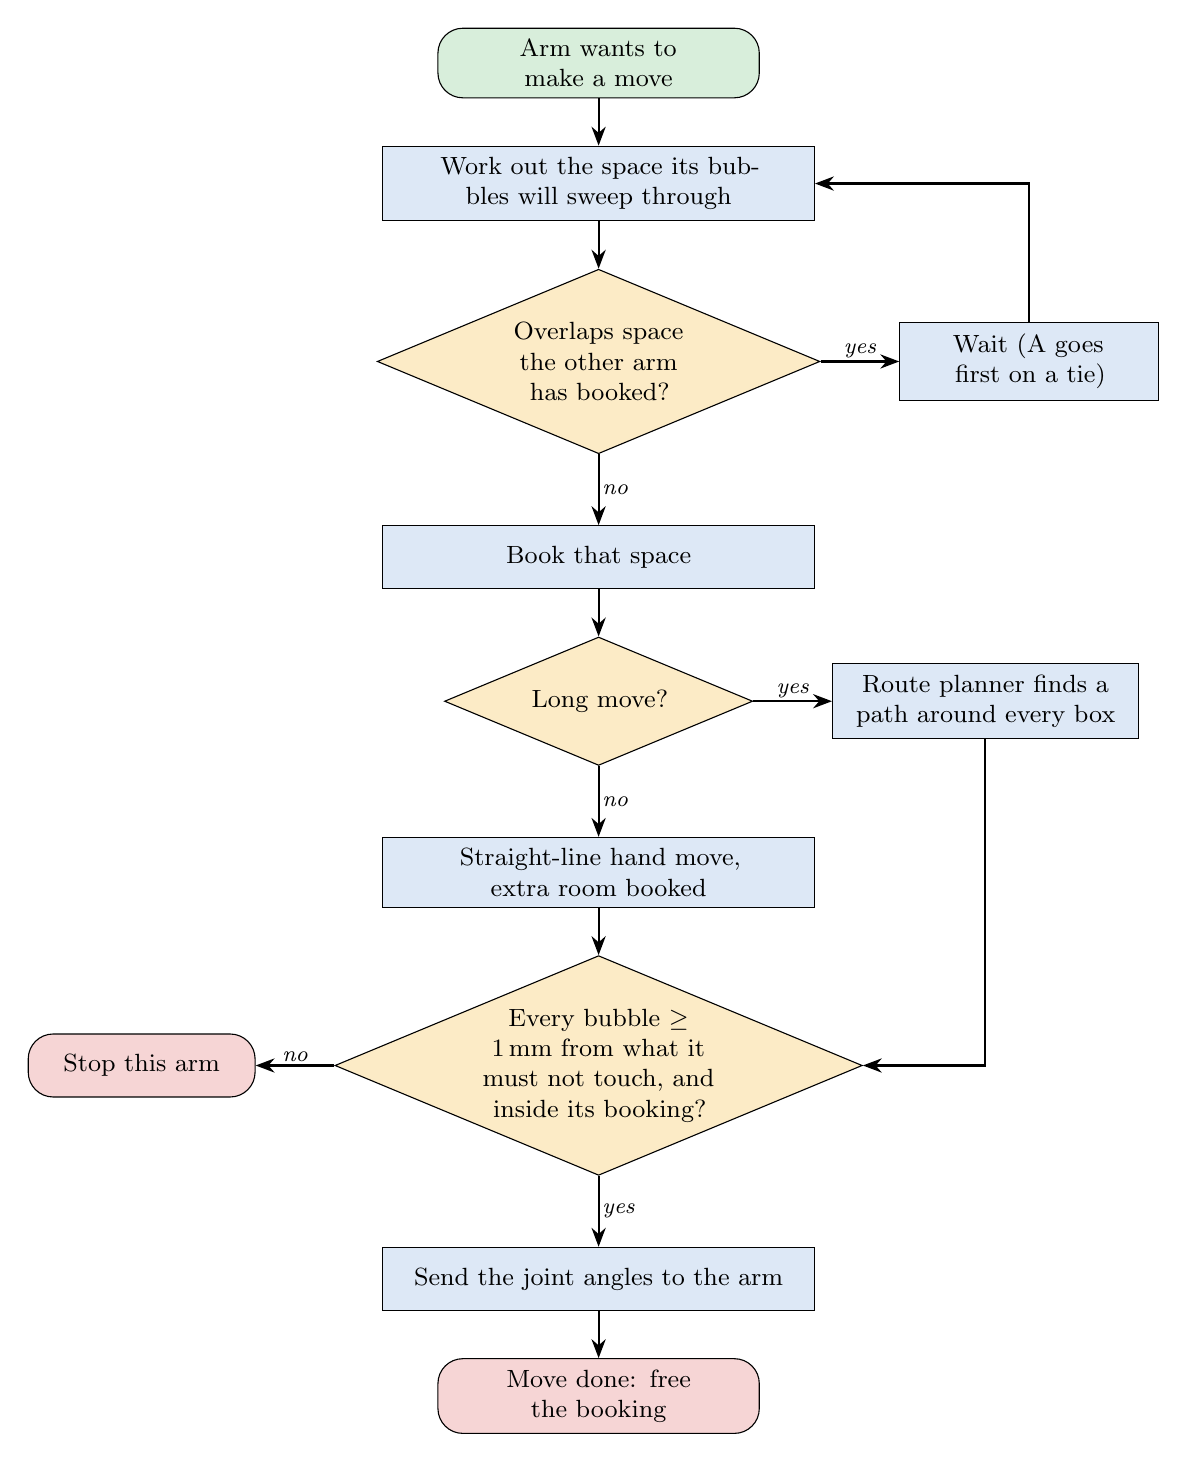
\begin{tikzpicture}[flow]
\node[start] (s) {Arm wants to make a move};
\node[step, below=of s] (b) {Work out the space its bubbles will sweep through};
\node[ask, below=of b] (q1) {Overlaps space the other arm has booked?};
\node[step=30mm, right=10mm of q1] (w) {Wait (A goes first on a tie)};
\node[step, below=of q1, yshift=-3mm] (k) {Book that space};
\node[ask, below=of k] (q2) {Long move?};
\node[step=36mm, right=10mm of q2] (p) {Route planner finds a path around every box};
\node[step, below=of q2, yshift=-3mm] (l) {Straight-line hand move, extra room booked};
\node[ask, below=of l] (q3) {Every bubble $\geq$ 1\,mm from what it must not touch, and inside its booking?};
\node[stop=26mm, left=10mm of q3] (x) {Stop this arm};
\node[step, below=of q3, yshift=-3mm] (m) {Send the joint angles to the arm};
\node[stop, below=of m] (e) {Move done: free the booking};
\draw[arr] (s)--(b); \draw[arr] (b)--(q1);
\draw[arr] (q1)-- node[lab, above]{yes} (w);
\draw[arr] (w.north) |- (b.east);
\draw[arr] (q1)-- node[lab, right]{no} (k);
\draw[arr] (k)--(q2);
\draw[arr] (q2)-- node[lab, above]{yes} (p);
\draw[arr] (p) |- (q3.east);
\draw[arr] (q2)-- node[lab, right]{no} (l);
\draw[arr] (l)--(q3);
\draw[arr] (q3)-- node[lab, right]{yes} (m);
\draw[arr] (q3)-- node[lab, above]{no} (x);
\draw[arr] (m)--(e);
\end{tikzpicture}
\caption{Planning a move and keeping it safe. The safety check runs again for every command, many times a second.}
\end{figure}

\subsection{Two arms, two models, and helping each other}

A small ``team leader'' program (the coordinator) keeps track of both builds:

\begin{itemize}
\item Each arm works through its own plan. When their moves do not overlap, both
      arms move at the same time.
\item When a step needs support, the building arm asks for help. The other arm
      finishes what it is doing, comes over, grips the model where the support
      plan says, and holds it. Only then does the builder carry its brick in.
\item When the brick is clicked in and the builder's hand is away, the helper lets
      go and returns to its own model.
\item If both arms ask for help at once, A is helped first and B's request is
      kept for next.
\end{itemize}

\begin{figure}[H]
\centering
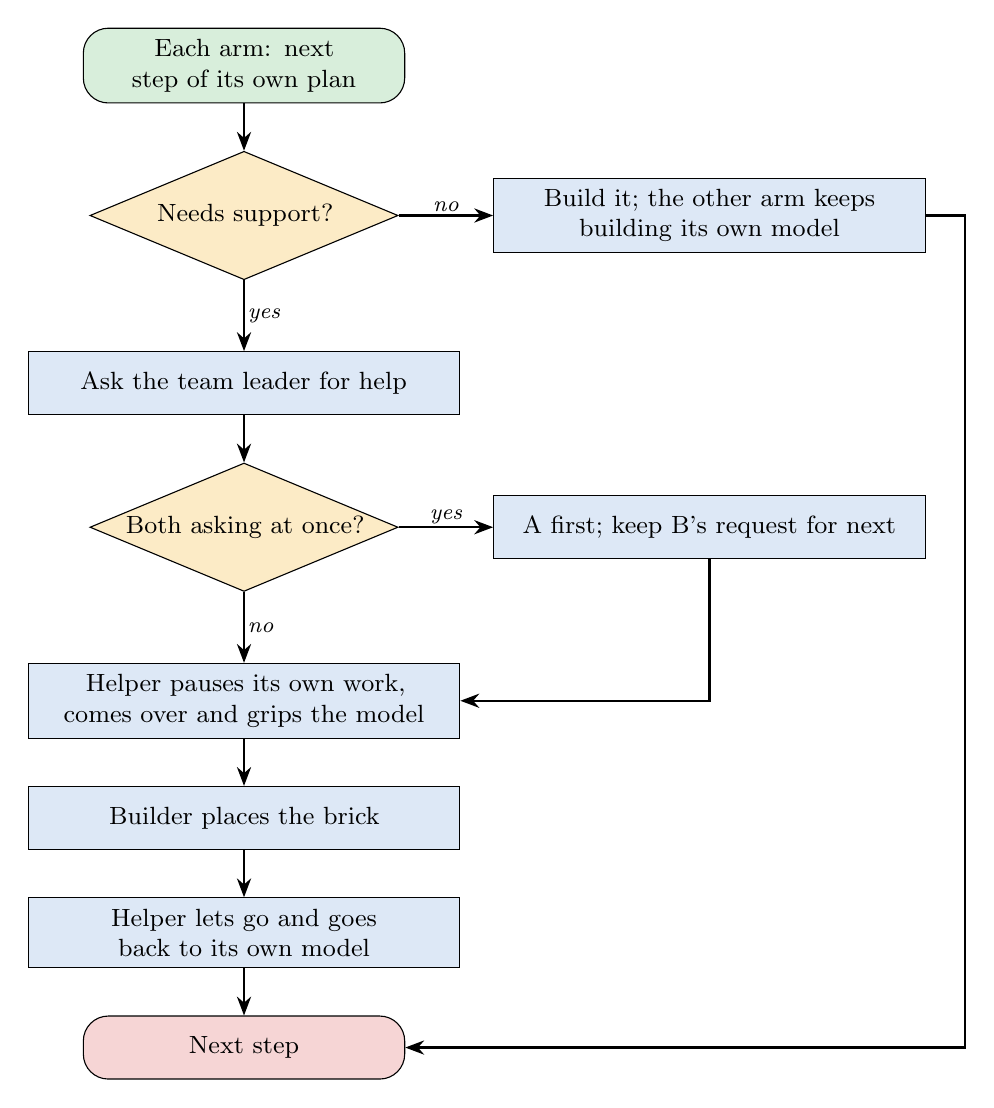
\begin{tikzpicture}[flow]
\node[start] (s) {Each arm: next step of its own plan};
\node[ask, below=of s] (q1) {Needs support?};
\node[step, right=12mm of q1] (n) {Build it; the other arm keeps building its own model};
\node[step, below=of q1, yshift=-3mm] (r) {Ask the team leader for help};
\node[ask, below=of r] (q2) {Both asking at once?};
\node[step, right=12mm of q2] (t) {A first; keep B's request for next};
\node[step, below=of q2, yshift=-3mm] (h) {Helper pauses its own work, comes over and grips the model};
\node[step, below=of h] (b) {Builder places the brick};
\node[step, below=of b] (l) {Helper lets go and goes back to its own model};
\node[stop, below=of l] (e) {Next step};
\draw[arr] (s)--(q1);
\draw[arr] (q1)-- node[lab, above]{no} (n);
\draw[arr] (n.east) -- ++(5mm,0) |- (e.east);
\draw[arr] (q1)-- node[lab, right]{yes} (r);
\draw[arr] (r)--(q2);
\draw[arr] (q2)-- node[lab, above]{yes} (t);
\draw[arr] (t) |- (h.east);
\draw[arr] (q2)-- node[lab, right]{no} (h);
\foreach \u/\v in {h/b,b/l,l/e} \draw[arr] (\u)--(\v);
\end{tikzpicture}
\caption{How the two arms share work and help each other.}
\end{figure}

\subsection{When is a step finished?}\label{sec:done}

A brick only counts as placed if it passes a strict check, called the
\textbf{snap check}, at the moment it should click in. The computer compares
where the brick really is with where the plan says it should be:

\begin{center}
\begin{tabular}{lc}
\toprule
What is measured & Must be less than \\
\midrule
Sideways distance from its spot & 2\,mm \\
Height above or below its spot & 1.5\,mm \\
Turned the wrong way & 5 degrees \\
Tipped over & 5 degrees \\
\bottomrule
\end{tabular}
\end{center}

If all four pass, the glue joints switch on and the step is complete. The arm
lets go, the team leader moves that arm on to its next brick, and any helper is
released. If any one fails, it is a \textbf{miss} and the build stops, so a
mistake is never hidden.

After the whole run, a separate \textbf{final check} reads the saved record of
the run. It confirms that every brick of both models was placed and is still
clicked in, that every support was really held, that no contact happened that
should not have, and that the code that ran is the code that was saved.

\begin{figure}[H]
\centering
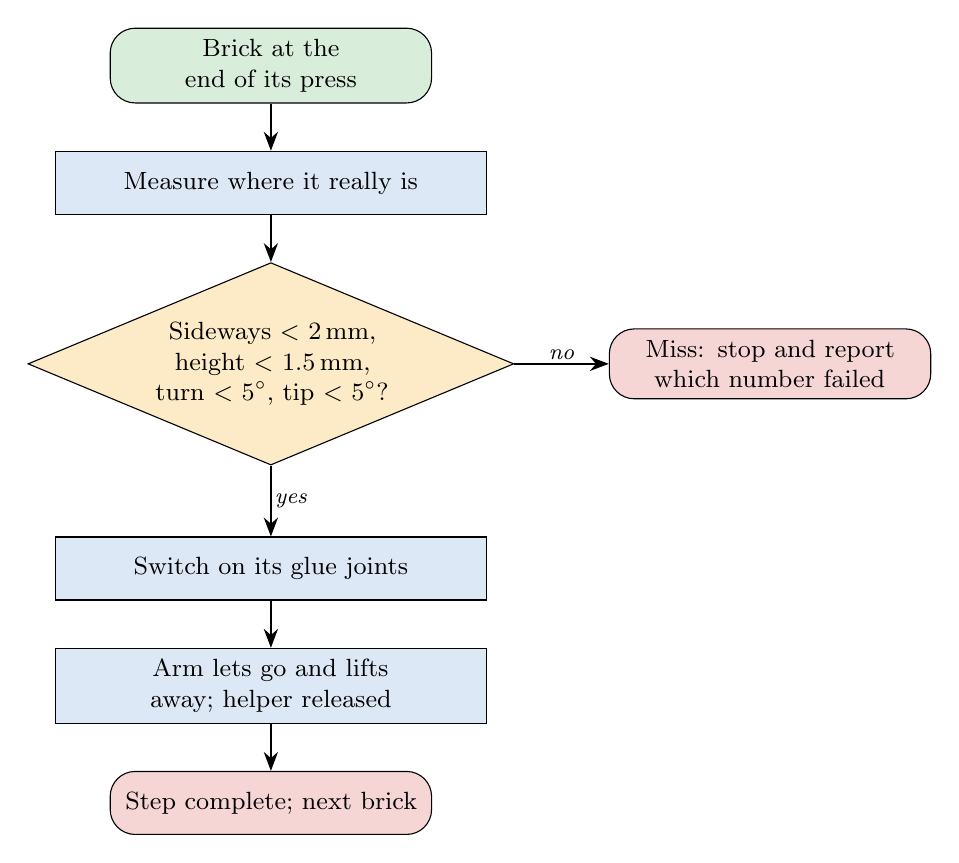
\begin{tikzpicture}[flow]
\node[start] (s) {Brick at the end of its press};
\node[step, below=of s] (m) {Measure where it really is};
\node[ask, below=of m, text width=34mm] (q) {Sideways $<$ 2\,mm, height $<$ 1.5\,mm, turn $<$ 5$^\circ$, tip $<$ 5$^\circ$?};
\node[stop, right=12mm of q] (x) {Miss: stop and report which number failed};
\node[step, below=of q, yshift=-3mm] (g) {Switch on its glue joints};
\node[step, below=of g] (o) {Arm lets go and lifts away; helper released};
\node[stop, below=of o] (e) {Step complete; next brick};
\draw[arr] (s)--(m); \draw[arr] (m)--(q);
\draw[arr] (q)-- node[lab, above]{no} (x);
\draw[arr] (q)-- node[lab, right]{yes} (g);
\draw[arr] (g)--(o); \draw[arr] (o)--(e);
\end{tikzpicture}
\caption{Deciding that a step is finished.}
\end{figure}

% =====================================================================
\section{What has been achieved so far}

\begin{center}
\begin{tabular}{p{0.38\linewidth}p{0.52\linewidth}}
\toprule
Run & Result \\
\midrule
Arch (arm A) and S3 tower (arm B) & Both finished, final check passed, both arms often moving at once (\texttt{dual\_arch\_s3\_012}, \texttt{014}, \texttt{015}). \\
Pyramid (A) and S3 (B) & Both finished, final check passed, after reordering the pyramid's small bricks (\texttt{dual\_pyramid\_s3\_006}). \\
Pyramid and S3 with real stud push (stud-fit) & The whole pyramid is built against the real stud push. S3 is built up to its second-to-last brick. On its last brick the press overloads one small 2-stud joint by a few percent, so that run does not pass yet. \\
\bottomrule
\end{tabular}
\end{center}

Videos of the runs are saved next to their results as \texttt{.mp4} files, and
every run can be replayed in a web browser.

\section{Words used in this report}

\begin{description}[leftmargin=2.6cm, style=nextline]
\item[Blueprint] The list of bricks that makes the model: type, position and direction.
\item[Plan] The blueprint put in build order, with how to grip and press each brick.
\item[Support] The other arm holding the model steady while a brick is pushed on.
\item[Simulation] A computer program that acts like the real world.
\item[Newton (N)] A unit of push; about the weight of a small apple.
\item[Feeder] The spot on the table where a brick waits to be picked up.
\item[Hover point] The spot just above a brick's place, where the arm pauses.
\item[Route planner] The program that finds a path for the arm around obstacles.
\item[Booking] Space an arm reserves before it moves, so the other arm keeps out.
\item[Snap check] The test that decides a brick is in the right place.
\item[Glue joint] The invisible link that holds a placed brick, and can break.
\end{description}

\end{document}
